% Created by tikzDevice version 0.12.6 on 2024-04-23 08:20:50
% !TEX encoding = UTF-8 Unicode
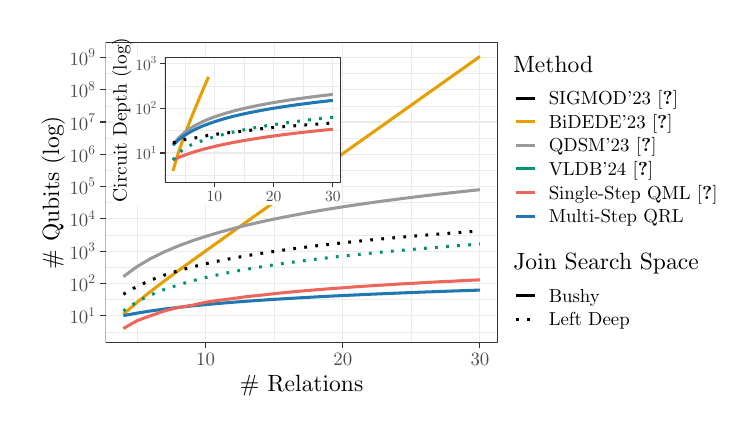
\begin{tikzpicture}[x=1pt,y=1pt]
\definecolor{fillColor}{RGB}{255,255,255}
\path[use as bounding box,fill=fillColor,fill opacity=0.00] (0,0) rectangle (251.96,138.58);
\begin{scope}
\path[clip] (  0.00,  0.00) rectangle (251.96,138.58);
\definecolor{drawColor}{RGB}{255,255,255}
\definecolor{fillColor}{RGB}{255,255,255}

\path[draw=drawColor,line width= 0.6pt,line join=round,line cap=round,fill=fillColor] (  0.00,  0.00) rectangle (251.96,138.58);
\end{scope}
\begin{scope}
\path[clip] (  5.50,  5.50) rectangle (246.46,133.08);
\definecolor{drawColor}{RGB}{255,255,255}
\definecolor{fillColor}{RGB}{255,255,255}

\path[draw=drawColor,line width= 0.4pt,line join=round,line cap=round,fill=fillColor] (  5.50,  5.50) rectangle (246.46,133.08);
\end{scope}
\begin{scope}
\path[clip] ( 28.13, 24.96) rectangle (169.86,133.08);
\definecolor{fillColor}{RGB}{255,255,255}

\path[fill=fillColor] ( 28.13, 24.96) rectangle (169.86,133.08);
\definecolor{drawColor}{gray}{0.92}

\path[draw=drawColor,line width= 0.2pt,line join=round] ( 28.13, 28.69) --
	(169.86, 28.69);

\path[draw=drawColor,line width= 0.2pt,line join=round] ( 28.13, 40.35) --
	(169.86, 40.35);

\path[draw=drawColor,line width= 0.2pt,line join=round] ( 28.13, 52.01) --
	(169.86, 52.01);

\path[draw=drawColor,line width= 0.2pt,line join=round] ( 28.13, 63.67) --
	(169.86, 63.67);

\path[draw=drawColor,line width= 0.2pt,line join=round] ( 28.13, 75.33) --
	(169.86, 75.33);

\path[draw=drawColor,line width= 0.2pt,line join=round] ( 28.13, 86.99) --
	(169.86, 86.99);

\path[draw=drawColor,line width= 0.2pt,line join=round] ( 28.13, 98.65) --
	(169.86, 98.65);

\path[draw=drawColor,line width= 0.2pt,line join=round] ( 28.13,110.31) --
	(169.86,110.31);

\path[draw=drawColor,line width= 0.2pt,line join=round] ( 28.13,121.97) --
	(169.86,121.97);

\path[draw=drawColor,line width= 0.2pt,line join=round] ( 39.53, 24.96) --
	( 39.53,133.08);

\path[draw=drawColor,line width= 0.2pt,line join=round] ( 89.09, 24.96) --
	( 89.09,133.08);

\path[draw=drawColor,line width= 0.2pt,line join=round] (138.64, 24.96) --
	(138.64,133.08);

\path[draw=drawColor,line width= 0.4pt,line join=round] ( 28.13, 34.52) --
	(169.86, 34.52);

\path[draw=drawColor,line width= 0.4pt,line join=round] ( 28.13, 46.18) --
	(169.86, 46.18);

\path[draw=drawColor,line width= 0.4pt,line join=round] ( 28.13, 57.84) --
	(169.86, 57.84);

\path[draw=drawColor,line width= 0.4pt,line join=round] ( 28.13, 69.50) --
	(169.86, 69.50);

\path[draw=drawColor,line width= 0.4pt,line join=round] ( 28.13, 81.16) --
	(169.86, 81.16);

\path[draw=drawColor,line width= 0.4pt,line join=round] ( 28.13, 92.82) --
	(169.86, 92.82);

\path[draw=drawColor,line width= 0.4pt,line join=round] ( 28.13,104.48) --
	(169.86,104.48);

\path[draw=drawColor,line width= 0.4pt,line join=round] ( 28.13,116.14) --
	(169.86,116.14);

\path[draw=drawColor,line width= 0.4pt,line join=round] ( 28.13,127.81) --
	(169.86,127.81);

\path[draw=drawColor,line width= 0.4pt,line join=round] ( 64.31, 24.96) --
	( 64.31,133.08);

\path[draw=drawColor,line width= 0.4pt,line join=round] (113.87, 24.96) --
	(113.87,133.08);

\path[draw=drawColor,line width= 0.4pt,line join=round] (163.42, 24.96) --
	(163.42,133.08);
\definecolor{drawColor}{RGB}{230,159,0}

\path[draw=drawColor,line width= 1.1pt,line join=round] ( 34.58, 35.00) --
	( 39.53, 39.36) --
	( 44.49, 43.33) --
	( 49.44, 47.10) --
	( 54.40, 50.76) --
	( 59.35, 54.35) --
	( 64.31, 57.90) --
	( 69.27, 61.44) --
	( 74.22, 64.96) --
	( 79.18, 68.48) --
	( 84.13, 72.00) --
	( 89.09, 75.51) --
	( 94.04, 79.02) --
	( 99.00, 82.53) --
	(103.95, 86.04) --
	(108.91, 89.55) --
	(113.87, 93.06) --
	(118.82, 96.57) --
	(123.78,100.08) --
	(128.73,103.59) --
	(133.69,107.10) --
	(138.64,110.61) --
	(143.60,114.12) --
	(148.55,117.63) --
	(153.51,121.15) --
	(158.47,124.66) --
	(163.42,128.17);
\definecolor{drawColor}{gray}{0.60}

\path[draw=drawColor,line width= 1.1pt,line join=round] ( 34.58, 48.62) --
	( 39.53, 52.25) --
	( 44.49, 55.17) --
	( 49.44, 57.60) --
	( 54.40, 59.69) --
	( 59.35, 61.53) --
	( 64.31, 63.16) --
	( 69.27, 64.64) --
	( 74.22, 65.98) --
	( 79.18, 67.22) --
	( 84.13, 68.36) --
	( 89.09, 69.42) --
	( 94.04, 70.41) --
	( 99.00, 71.34) --
	(103.95, 72.22) --
	(108.91, 73.05) --
	(113.87, 73.83) --
	(118.82, 74.58) --
	(123.78, 75.29) --
	(128.73, 75.97) --
	(133.69, 76.62) --
	(138.64, 77.25) --
	(143.60, 77.84) --
	(148.55, 78.42) --
	(153.51, 78.98) --
	(158.47, 79.51) --
	(163.42, 80.03);
\definecolor{drawColor}{RGB}{31,120,180}

\path[draw=drawColor,line width= 1.1pt,line join=round] ( 34.58, 34.52) --
	( 39.53, 35.44) --
	( 44.49, 36.22) --
	( 49.44, 36.90) --
	( 54.40, 37.49) --
	( 59.35, 38.03) --
	( 64.31, 38.51) --
	( 69.27, 38.95) --
	( 74.22, 39.36) --
	( 79.18, 39.73) --
	( 84.13, 40.08) --
	( 89.09, 40.41) --
	( 94.04, 40.71) --
	( 99.00, 41.00) --
	(103.95, 41.28) --
	(108.91, 41.54) --
	(113.87, 41.78) --
	(118.82, 42.02) --
	(123.78, 42.25) --
	(128.73, 42.46) --
	(133.69, 42.67) --
	(138.64, 42.87) --
	(143.60, 43.06) --
	(148.55, 43.24) --
	(153.51, 43.42) --
	(158.47, 43.59) --
	(163.42, 43.76);
\definecolor{drawColor}{RGB}{0,0,0}

\path[draw=drawColor,line width= 1.1pt,dash pattern=on 1pt off 3pt ,line join=round] ( 34.58, 42.25) --
	( 39.53, 45.11) --
	( 44.49, 47.35) --
	( 49.44, 49.18) --
	( 54.40, 50.74) --
	( 59.35, 52.08) --
	( 64.31, 53.27) --
	( 69.27, 54.34) --
	( 74.22, 55.30) --
	( 79.18, 56.18) --
	( 84.13, 56.99) --
	( 89.09, 57.74) --
	( 94.04, 58.44) --
	( 99.00, 59.09) --
	(103.95, 59.71) --
	(108.91, 60.29) --
	(113.87, 60.83) --
	(118.82, 61.35) --
	(123.78, 61.85) --
	(128.73, 62.32) --
	(133.69, 62.77) --
	(138.64, 63.20) --
	(143.60, 63.61) --
	(148.55, 64.01) --
	(153.51, 64.39) --
	(158.47, 64.76) --
	(163.42, 65.11);
\definecolor{drawColor}{RGB}{237,102,90}

\path[draw=drawColor,line width= 1.1pt,line join=round] ( 34.58, 29.88) --
	( 39.53, 32.71) --
	( 44.49, 34.52) --
	( 49.44, 36.22) --
	( 54.40, 37.49) --
	( 59.35, 38.27) --
	( 64.31, 39.36) --
	( 69.27, 40.08) --
	( 74.22, 40.71) --
	( 79.18, 41.41) --
	( 84.13, 41.90) --
	( 89.09, 42.46) --
	( 94.04, 42.96) --
	( 99.00, 43.42) --
	(103.95, 43.84) --
	(108.91, 44.22) --
	(113.87, 44.58) --
	(118.82, 44.98) --
	(123.78, 45.29) --
	(128.73, 45.59) --
	(133.69, 45.92) --
	(138.64, 46.18) --
	(143.60, 46.47) --
	(148.55, 46.75) --
	(153.51, 46.97) --
	(158.47, 47.23) --
	(163.42, 47.47);
\definecolor{drawColor}{RGB}{0,147,113}

\path[draw=drawColor,line width= 1.1pt,dash pattern=on 1pt off 3pt ,line join=round] ( 34.58, 36.22) --
	( 39.53, 39.55) --
	( 44.49, 42.02) --
	( 49.44, 44.00) --
	( 54.40, 45.64) --
	( 59.35, 47.06) --
	( 64.31, 48.30) --
	( 69.27, 49.40) --
	( 74.22, 50.40) --
	( 79.18, 51.30) --
	( 84.13, 52.13) --
	( 89.09, 52.90) --
	( 94.04, 53.61) --
	( 99.00, 54.28) --
	(103.95, 54.90) --
	(108.91, 55.49) --
	(113.87, 56.05) --
	(118.82, 56.57) --
	(123.78, 57.07) --
	(128.73, 57.55) --
	(133.69, 58.01) --
	(138.64, 58.44) --
	(143.60, 58.86) --
	(148.55, 59.26) --
	(153.51, 59.65) --
	(158.47, 60.02) --
	(163.42, 60.38);
\definecolor{drawColor}{gray}{0.20}

\path[draw=drawColor,line width= 0.4pt,line join=round,line cap=round] ( 28.13, 24.96) rectangle (169.86,133.08);
\end{scope}
\begin{scope}
\path[clip] (  0.00,  0.00) rectangle (251.96,138.58);
\definecolor{drawColor}{gray}{0.30}

\node[text=drawColor,anchor=base west,inner sep=0pt, outer sep=0pt, scale=  0.68] at ( 15.13, 31.60) {10};

\node[text=drawColor,anchor=base west,inner sep=0pt, outer sep=0pt, scale=  0.48] at ( 21.93, 34.38) {1};

\node[text=drawColor,anchor=base west,inner sep=0pt, outer sep=0pt, scale=  0.68] at ( 15.13, 43.26) {10};

\node[text=drawColor,anchor=base west,inner sep=0pt, outer sep=0pt, scale=  0.48] at ( 21.93, 46.04) {2};

\node[text=drawColor,anchor=base west,inner sep=0pt, outer sep=0pt, scale=  0.68] at ( 15.13, 54.92) {10};

\node[text=drawColor,anchor=base west,inner sep=0pt, outer sep=0pt, scale=  0.48] at ( 21.93, 57.70) {3};

\node[text=drawColor,anchor=base west,inner sep=0pt, outer sep=0pt, scale=  0.68] at ( 15.13, 66.58) {10};

\node[text=drawColor,anchor=base west,inner sep=0pt, outer sep=0pt, scale=  0.48] at ( 21.93, 69.36) {4};

\node[text=drawColor,anchor=base west,inner sep=0pt, outer sep=0pt, scale=  0.68] at ( 15.13, 78.24) {10};

\node[text=drawColor,anchor=base west,inner sep=0pt, outer sep=0pt, scale=  0.48] at ( 21.93, 81.02) {5};

\node[text=drawColor,anchor=base west,inner sep=0pt, outer sep=0pt, scale=  0.68] at ( 15.13, 89.91) {10};

\node[text=drawColor,anchor=base west,inner sep=0pt, outer sep=0pt, scale=  0.48] at ( 21.93, 92.69) {6};

\node[text=drawColor,anchor=base west,inner sep=0pt, outer sep=0pt, scale=  0.68] at ( 15.13,101.57) {10};

\node[text=drawColor,anchor=base west,inner sep=0pt, outer sep=0pt, scale=  0.48] at ( 21.93,104.35) {7};

\node[text=drawColor,anchor=base west,inner sep=0pt, outer sep=0pt, scale=  0.68] at ( 15.13,113.23) {10};

\node[text=drawColor,anchor=base west,inner sep=0pt, outer sep=0pt, scale=  0.48] at ( 21.93,116.01) {8};

\node[text=drawColor,anchor=base west,inner sep=0pt, outer sep=0pt, scale=  0.68] at ( 15.13,124.89) {10};

\node[text=drawColor,anchor=base west,inner sep=0pt, outer sep=0pt, scale=  0.48] at ( 21.93,127.67) {9};
\end{scope}
\begin{scope}
\path[clip] (  0.00,  0.00) rectangle (251.96,138.58);
\definecolor{drawColor}{gray}{0.20}

\path[draw=drawColor,line width= 0.4pt,line join=round] ( 26.01, 34.52) --
	( 28.13, 34.52);

\path[draw=drawColor,line width= 0.4pt,line join=round] ( 26.01, 46.18) --
	( 28.13, 46.18);

\path[draw=drawColor,line width= 0.4pt,line join=round] ( 26.01, 57.84) --
	( 28.13, 57.84);

\path[draw=drawColor,line width= 0.4pt,line join=round] ( 26.01, 69.50) --
	( 28.13, 69.50);

\path[draw=drawColor,line width= 0.4pt,line join=round] ( 26.01, 81.16) --
	( 28.13, 81.16);

\path[draw=drawColor,line width= 0.4pt,line join=round] ( 26.01, 92.82) --
	( 28.13, 92.82);

\path[draw=drawColor,line width= 0.4pt,line join=round] ( 26.01,104.48) --
	( 28.13,104.48);

\path[draw=drawColor,line width= 0.4pt,line join=round] ( 26.01,116.14) --
	( 28.13,116.14);

\path[draw=drawColor,line width= 0.4pt,line join=round] ( 26.01,127.81) --
	( 28.13,127.81);
\end{scope}
\begin{scope}
\path[clip] (  0.00,  0.00) rectangle (251.96,138.58);
\definecolor{drawColor}{gray}{0.20}

\path[draw=drawColor,line width= 0.4pt,line join=round] ( 64.31, 22.84) --
	( 64.31, 24.96);

\path[draw=drawColor,line width= 0.4pt,line join=round] (113.87, 22.84) --
	(113.87, 24.96);

\path[draw=drawColor,line width= 0.4pt,line join=round] (163.42, 22.84) --
	(163.42, 24.96);
\end{scope}
\begin{scope}
\path[clip] (  0.00,  0.00) rectangle (251.96,138.58);
\definecolor{drawColor}{gray}{0.30}

\node[text=drawColor,anchor=base,inner sep=0pt, outer sep=0pt, scale=  0.68] at ( 64.31, 16.45) {10};

\node[text=drawColor,anchor=base,inner sep=0pt, outer sep=0pt, scale=  0.68] at (113.87, 16.45) {20};

\node[text=drawColor,anchor=base,inner sep=0pt, outer sep=0pt, scale=  0.68] at (163.42, 16.45) {30};
\end{scope}
\begin{scope}
\path[clip] (  0.00,  0.00) rectangle (251.96,138.58);
\definecolor{drawColor}{RGB}{0,0,0}

\node[text=drawColor,anchor=base,inner sep=0pt, outer sep=0pt, scale=  0.85] at ( 99.00,  7.15) {\# Relations};
\end{scope}
\begin{scope}
\path[clip] (  0.00,  0.00) rectangle (251.96,138.58);
\definecolor{drawColor}{RGB}{0,0,0}

\node[text=drawColor,rotate= 90.00,anchor=base,inner sep=0pt, outer sep=0pt, scale=  0.85] at ( 11.35, 79.02) {\# Qubits (log)};
\end{scope}
\begin{scope}
\path[clip] (  0.00,  0.00) rectangle (251.96,138.58);
\definecolor{fillColor}{RGB}{255,255,255}

\path[fill=fillColor] (178.36, 66.20) rectangle (246.46,129.17);
\end{scope}
\begin{scope}
\path[clip] (  0.00,  0.00) rectangle (251.96,138.58);
\definecolor{drawColor}{RGB}{0,0,0}

\node[text=drawColor,anchor=base west,inner sep=0pt, outer sep=0pt, scale=  0.85] at (175.52,122.49) {Method};
\end{scope}
\begin{scope}
\path[clip] (  0.00,  0.00) rectangle (251.96,138.58);
\definecolor{fillColor}{RGB}{255,255,255}

\path[fill=fillColor] (175.52,108.88) rectangle (184.05,117.41);
\end{scope}
\begin{scope}
\path[clip] (  0.00,  0.00) rectangle (251.96,138.58);
\definecolor{drawColor}{RGB}{0,0,0}

\path[draw=drawColor,line width= 1.1pt,line join=round] (176.37,113.15) -- (183.20,113.15);
\end{scope}
\begin{scope}
\path[clip] (  0.00,  0.00) rectangle (251.96,138.58);
\definecolor{fillColor}{RGB}{255,255,255}

\path[fill=fillColor] (175.52,100.34) rectangle (184.05,108.88);
\end{scope}
\begin{scope}
\path[clip] (  0.00,  0.00) rectangle (251.96,138.58);
\definecolor{drawColor}{RGB}{230,159,0}

\path[draw=drawColor,line width= 1.1pt,line join=round] (176.37,104.61) -- (183.20,104.61);
\end{scope}
\begin{scope}
\path[clip] (  0.00,  0.00) rectangle (251.96,138.58);
\definecolor{fillColor}{RGB}{255,255,255}

\path[fill=fillColor] (175.52, 91.81) rectangle (184.05,100.34);
\end{scope}
\begin{scope}
\path[clip] (  0.00,  0.00) rectangle (251.96,138.58);
\definecolor{drawColor}{gray}{0.60}

\path[draw=drawColor,line width= 1.1pt,line join=round] (176.37, 96.07) -- (183.20, 96.07);
\end{scope}
\begin{scope}
\path[clip] (  0.00,  0.00) rectangle (251.96,138.58);
\definecolor{fillColor}{RGB}{255,255,255}

\path[fill=fillColor] (175.52, 83.27) rectangle (184.05, 91.81);
\end{scope}
\begin{scope}
\path[clip] (  0.00,  0.00) rectangle (251.96,138.58);
\definecolor{drawColor}{RGB}{0,147,113}

\path[draw=drawColor,line width= 1.1pt,line join=round] (176.37, 87.54) -- (183.20, 87.54);
\end{scope}
\begin{scope}
\path[clip] (  0.00,  0.00) rectangle (251.96,138.58);
\definecolor{fillColor}{RGB}{255,255,255}

\path[fill=fillColor] (175.52, 74.74) rectangle (184.05, 83.27);
\end{scope}
\begin{scope}
\path[clip] (  0.00,  0.00) rectangle (251.96,138.58);
\definecolor{drawColor}{RGB}{237,102,90}

\path[draw=drawColor,line width= 1.1pt,line join=round] (176.37, 79.00) -- (183.20, 79.00);
\end{scope}
\begin{scope}
\path[clip] (  0.00,  0.00) rectangle (251.96,138.58);
\definecolor{fillColor}{RGB}{255,255,255}

\path[fill=fillColor] (175.52, 66.20) rectangle (184.05, 74.74);
\end{scope}
\begin{scope}
\path[clip] (  0.00,  0.00) rectangle (251.96,138.58);
\definecolor{drawColor}{RGB}{31,120,180}

\path[draw=drawColor,line width= 1.1pt,line join=round] (176.37, 70.47) -- (183.20, 70.47);
\end{scope}
\begin{scope}
\path[clip] (  0.00,  0.00) rectangle (251.96,138.58);
\definecolor{drawColor}{RGB}{0,0,0}

\node[text=drawColor,anchor=base west,inner sep=0pt, outer sep=0pt, scale=  0.68] at (188.30,110.80) {SIGMOD'23~\cite{schoenberger23}};
\end{scope}
\begin{scope}
\path[clip] (  0.00,  0.00) rectangle (251.96,138.58);
\definecolor{drawColor}{RGB}{0,0,0}

\node[text=drawColor,anchor=base west,inner sep=0pt, outer sep=0pt, scale=  0.68] at (188.30,102.27) {BiDEDE'23~\cite{nayak23}};
\end{scope}
\begin{scope}
\path[clip] (  0.00,  0.00) rectangle (251.96,138.58);
\definecolor{drawColor}{RGB}{0,0,0}

\node[text=drawColor,anchor=base west,inner sep=0pt, outer sep=0pt, scale=  0.68] at (188.30, 93.73) {QDSM'23~\cite{schoenberger23:qdsm}};
\end{scope}
\begin{scope}
\path[clip] (  0.00,  0.00) rectangle (251.96,138.58);
\definecolor{drawColor}{RGB}{0,0,0}

\node[text=drawColor,anchor=base west,inner sep=0pt, outer sep=0pt, scale=  0.68] at (188.30, 85.20) {VLDB'24~\cite{schoenberger24}};
\end{scope}
\begin{scope}
\path[clip] (  0.00,  0.00) rectangle (251.96,138.58);
\definecolor{drawColor}{RGB}{0,0,0}

\node[text=drawColor,anchor=base west,inner sep=0pt, outer sep=0pt, scale=  0.68] at (188.30, 76.66) {Single-Step QML~\cite{winker23}};
\end{scope}
\begin{scope}
\path[clip] (  0.00,  0.00) rectangle (251.96,138.58);
\definecolor{drawColor}{RGB}{0,0,0}

\node[text=drawColor,anchor=base west,inner sep=0pt, outer sep=0pt, scale=  0.68] at (188.30, 68.13) {Multi-Step QRL};
\end{scope}
\begin{scope}
\path[clip] (  0.00,  0.00) rectangle (251.96,138.58);
\definecolor{fillColor}{RGB}{255,255,255}

\path[fill=fillColor] (178.36, 28.87) rectangle (239.62, 57.70);
\end{scope}
\begin{scope}
\path[clip] (  0.00,  0.00) rectangle (251.96,138.58);
\definecolor{drawColor}{RGB}{0,0,0}

\node[text=drawColor,anchor=base west,inner sep=0pt, outer sep=0pt, scale=  0.85] at (175.52, 51.02) {Join Search Space};
\end{scope}
\begin{scope}
\path[clip] (  0.00,  0.00) rectangle (251.96,138.58);
\definecolor{fillColor}{RGB}{255,255,255}

\path[fill=fillColor] (175.52, 37.41) rectangle (184.05, 45.94);
\end{scope}
\begin{scope}
\path[clip] (  0.00,  0.00) rectangle (251.96,138.58);
\definecolor{drawColor}{RGB}{0,0,0}

\path[draw=drawColor,line width= 1.1pt,line join=round] (176.37, 41.67) -- (183.20, 41.67);
\end{scope}
\begin{scope}
\path[clip] (  0.00,  0.00) rectangle (251.96,138.58);
\definecolor{fillColor}{RGB}{255,255,255}

\path[fill=fillColor] (175.52, 28.87) rectangle (184.05, 37.41);
\end{scope}
\begin{scope}
\path[clip] (  0.00,  0.00) rectangle (251.96,138.58);
\definecolor{drawColor}{RGB}{0,0,0}

\path[draw=drawColor,line width= 1.1pt,dash pattern=on 1pt off 3pt ,line join=round] (176.37, 33.14) -- (183.20, 33.14);
\end{scope}
\begin{scope}
\path[clip] (  0.00,  0.00) rectangle (251.96,138.58);
\definecolor{drawColor}{RGB}{0,0,0}

\node[text=drawColor,anchor=base west,inner sep=0pt, outer sep=0pt, scale=  0.68] at (188.30, 39.33) {Bushy};
\end{scope}
\begin{scope}
\path[clip] (  0.00,  0.00) rectangle (251.96,138.58);
\definecolor{drawColor}{RGB}{0,0,0}

\node[text=drawColor,anchor=base west,inner sep=0pt, outer sep=0pt, scale=  0.68] at (188.30, 30.80) {Left Deep};
\end{scope}
\begin{scope}
\path[clip] ( 30.97, 74.70) rectangle (113.17,127.67);
\definecolor{drawColor}{RGB}{255,255,255}
\definecolor{fillColor}{RGB}{255,255,255}

\path[draw=drawColor,line width= 0.4pt,line join=round,line cap=round,fill=fillColor] ( 30.97, 74.70) rectangle (113.17,127.67);
\end{scope}
\begin{scope}
\path[clip] ( 49.61, 82.79) rectangle (113.17,127.67);

\path[] ( 49.61, 82.79) rectangle (113.17,127.67);
\definecolor{drawColor}{gray}{0.92}

\path[draw=drawColor,line width= 0.2pt,line join=round] ( 49.61, 85.20) --
	(113.17, 85.20);

\path[draw=drawColor,line width= 0.2pt,line join=round] ( 49.61,101.37) --
	(113.17,101.37);

\path[draw=drawColor,line width= 0.2pt,line join=round] ( 49.61,117.55) --
	(113.17,117.55);

\path[draw=drawColor,line width= 0.2pt,line join=round] ( 56.78, 82.79) --
	( 56.78,127.67);

\path[draw=drawColor,line width= 0.2pt,line join=round] ( 78.18, 82.79) --
	( 78.18,127.67);

\path[draw=drawColor,line width= 0.2pt,line join=round] ( 99.58, 82.79) --
	( 99.58,127.67);

\path[draw=drawColor,line width= 0.4pt,line join=round] ( 49.61, 93.29) --
	(113.17, 93.29);

\path[draw=drawColor,line width= 0.4pt,line join=round] ( 49.61,109.46) --
	(113.17,109.46);

\path[draw=drawColor,line width= 0.4pt,line join=round] ( 49.61,125.63) --
	(113.17,125.63);

\path[draw=drawColor,line width= 0.4pt,line join=round] ( 67.48, 82.79) --
	( 67.48,127.67);

\path[draw=drawColor,line width= 0.4pt,line join=round] ( 88.88, 82.79) --
	( 88.88,127.67);

\path[draw=drawColor,line width= 0.4pt,line join=round] (110.28, 82.79) --
	(110.28,127.67);
\definecolor{drawColor}{RGB}{230,159,0}

\path[draw=drawColor,line width= 1.1pt,line join=round] ( 52.50, 86.85) --
	( 54.64, 93.96) --
	( 56.78,100.00) --
	( 58.92,105.51) --
	( 61.06,110.74) --
	( 63.20,115.81) --
	( 65.34,120.79);
\definecolor{drawColor}{gray}{0.60}

\path[draw=drawColor,line width= 1.1pt,line join=round] ( 52.50, 96.14) --
	( 54.64, 98.83) --
	( 56.78,100.77) --
	( 58.92,102.29) --
	( 61.06,103.53) --
	( 63.20,104.59) --
	( 65.34,105.51) --
	( 67.48,106.33) --
	( 69.62,107.06) --
	( 71.76,107.72) --
	( 73.90,108.32) --
	( 76.04,108.88) --
	( 78.18,109.39) --
	( 80.32,109.87) --
	( 82.46,110.32) --
	( 84.60,110.74) --
	( 86.74,111.14) --
	( 88.88,111.52) --
	( 91.02,111.87) --
	( 93.16,112.21) --
	( 95.30,112.54) --
	( 97.44,112.85) --
	( 99.58,113.15) --
	(101.72,113.43) --
	(103.86,113.71) --
	(106.00,113.97) --
	(108.14,114.22) --
	(110.28,114.47);
\definecolor{drawColor}{RGB}{237,102,90}

\path[draw=drawColor,line width= 1.1pt,line join=round] ( 52.50, 90.78) --
	( 54.64, 91.72) --
	( 56.78, 92.55) --
	( 58.92, 93.29) --
	( 61.06, 93.96) --
	( 63.20, 94.57) --
	( 65.34, 95.13) --
	( 67.48, 95.65) --
	( 69.62, 96.14) --
	( 71.76, 96.59) --
	( 73.90, 97.02) --
	( 76.04, 97.42) --
	( 78.18, 97.80) --
	( 80.32, 98.16) --
	( 82.46, 98.50) --
	( 84.60, 98.83) --
	( 86.74, 99.14) --
	( 88.88, 99.44) --
	( 91.02, 99.72) --
	( 93.16,100.00) --
	( 95.30,100.26) --
	( 97.44,100.52) --
	( 99.58,100.77) --
	(101.72,101.00) --
	(103.86,101.24) --
	(106.00,101.46) --
	(108.14,101.67) --
	(110.28,101.88);
\definecolor{drawColor}{RGB}{31,120,180}

\path[draw=drawColor,line width= 1.1pt,line join=round] ( 52.50, 96.14) --
	( 54.64, 98.16) --
	( 56.78, 99.72) --
	( 58.92,101.00) --
	( 61.06,102.09) --
	( 63.20,103.03) --
	( 65.34,103.85) --
	( 67.48,104.59) --
	( 69.62,105.26) --
	( 71.76,105.87) --
	( 73.90,106.44) --
	( 76.04,106.96) --
	( 78.18,107.44) --
	( 80.32,107.89) --
	( 82.46,108.32) --
	( 84.60,108.72) --
	( 86.74,109.10) --
	( 88.88,109.46) --
	( 91.02,109.80) --
	( 93.16,110.13) --
	( 95.30,110.44) --
	( 97.44,110.74) --
	( 99.58,111.03) --
	(101.72,111.30) --
	(103.86,111.57) --
	(106.00,111.82) --
	(108.14,112.07) --
	(110.28,112.31);
\definecolor{drawColor}{RGB}{0,0,0}

\path[draw=drawColor,line width= 1.1pt,dash pattern=on 1pt off 3pt ,line join=round] ( 52.50, 97.02) --
	( 54.64, 97.42) --
	( 56.78, 98.16) --
	( 58.92, 98.50) --
	( 61.06, 98.83) --
	( 63.20, 99.14) --
	( 65.34, 99.72) --
	( 67.48,100.00) --
	( 69.62,100.26) --
	( 71.76,100.52) --
	( 73.90,100.77) --
	( 76.04,101.00) --
	( 78.18,101.24) --
	( 80.32,101.46) --
	( 82.46,101.88) --
	( 84.60,102.09) --
	( 86.74,102.29) --
	( 88.88,102.48) --
	( 91.02,102.67) --
	( 93.16,102.85) --
	( 95.30,103.03) --
	( 97.44,103.20) --
	( 99.58,103.37) --
	(101.72,103.53) --
	(103.86,103.69) --
	(106.00,103.85) --
	(108.14,104.01) --
	(110.28,104.16);
\definecolor{drawColor}{RGB}{0,147,113}

\path[draw=drawColor,line width= 1.1pt,dash pattern=on 1pt off 3pt ,line join=round] ( 52.50, 90.78) --
	( 54.64, 93.29) --
	( 56.78, 95.13) --
	( 58.92, 96.14) --
	( 61.06, 97.02) --
	( 63.20, 97.80) --
	( 65.34, 98.50) --
	( 67.48, 99.14) --
	( 69.62, 99.72) --
	( 71.76,100.26) --
	( 73.90,100.77) --
	( 76.04,101.24) --
	( 78.18,101.67) --
	( 80.32,102.09) --
	( 82.46,102.48) --
	( 84.60,102.85) --
	( 86.74,103.20) --
	( 88.88,103.53) --
	( 91.02,103.85) --
	( 93.16,104.16) --
	( 95.30,104.45) --
	( 97.44,104.73) --
	( 99.58,105.00) --
	(101.72,105.26) --
	(103.86,105.51) --
	(106.00,105.76) --
	(108.14,105.99) --
	(110.28,106.22);
\definecolor{drawColor}{gray}{0.20}

\path[draw=drawColor,line width= 0.4pt,line join=round,line cap=round] ( 49.61, 82.79) rectangle (113.17,127.67);
\end{scope}
\begin{scope}
\path[clip] (  0.00,  0.00) rectangle (251.96,138.58);
\definecolor{drawColor}{gray}{0.30}

\node[text=drawColor,anchor=base west,inner sep=0pt, outer sep=0pt, scale=  0.56] at ( 38.90, 90.89) {10};

\node[text=drawColor,anchor=base west,inner sep=0pt, outer sep=0pt, scale=  0.39] at ( 44.50, 93.18) {1};

\node[text=drawColor,anchor=base west,inner sep=0pt, outer sep=0pt, scale=  0.56] at ( 38.90,107.06) {10};

\node[text=drawColor,anchor=base west,inner sep=0pt, outer sep=0pt, scale=  0.39] at ( 44.50,109.35) {2};

\node[text=drawColor,anchor=base west,inner sep=0pt, outer sep=0pt, scale=  0.56] at ( 38.90,123.23) {10};

\node[text=drawColor,anchor=base west,inner sep=0pt, outer sep=0pt, scale=  0.39] at ( 44.50,125.52) {3};
\end{scope}
\begin{scope}
\path[clip] (  0.00,  0.00) rectangle (251.96,138.58);
\definecolor{drawColor}{gray}{0.20}

\path[draw=drawColor,line width= 0.4pt,line join=round] ( 47.86, 93.29) --
	( 49.61, 93.29);

\path[draw=drawColor,line width= 0.4pt,line join=round] ( 47.86,109.46) --
	( 49.61,109.46);

\path[draw=drawColor,line width= 0.4pt,line join=round] ( 47.86,125.63) --
	( 49.61,125.63);
\end{scope}
\begin{scope}
\path[clip] (  0.00,  0.00) rectangle (251.96,138.58);
\definecolor{drawColor}{gray}{0.20}

\path[draw=drawColor,line width= 0.4pt,line join=round] ( 67.48, 81.04) --
	( 67.48, 82.79);

\path[draw=drawColor,line width= 0.4pt,line join=round] ( 88.88, 81.04) --
	( 88.88, 82.79);

\path[draw=drawColor,line width= 0.4pt,line join=round] (110.28, 81.04) --
	(110.28, 82.79);
\end{scope}
\begin{scope}
\path[clip] (  0.00,  0.00) rectangle (251.96,138.58);
\definecolor{drawColor}{gray}{0.30}

\node[text=drawColor,anchor=base,inner sep=0pt, outer sep=0pt, scale=  0.56] at ( 67.48, 75.78) {10};

\node[text=drawColor,anchor=base,inner sep=0pt, outer sep=0pt, scale=  0.56] at ( 88.88, 75.78) {20};

\node[text=drawColor,anchor=base,inner sep=0pt, outer sep=0pt, scale=  0.56] at (110.28, 75.78) {30};
\end{scope}
\begin{scope}
\path[clip] (  0.00,  0.00) rectangle (251.96,138.58);
\definecolor{drawColor}{RGB}{0,0,0}

\node[text=drawColor,rotate= 90.00,anchor=base,inner sep=0pt, outer sep=0pt, scale=  0.70] at ( 35.79,105.23) {Circuit Depth (log)};
\end{scope}
\end{tikzpicture}
